%%
%% This is file `mcmthesis-demo.tex',
%% generated with the docstrip utility.
%%
%% The original source files were:
%%
%% mcmthesis.dtx  (with options: `demo')
%% 
%% -----------------------------------
%% 
%% This is a generated file.
%% 
%% Copyright (C)
%%     2010 -- 2015 by Zhaoli Wang
%%     2014 -- 2016 by Liam Huang
%% 
%% This work may be distributed and/or modified under the
%% conditions of the LaTeX Project Public License, either version 1.3
%% of this license or (at your option) any later version.
%% The latest version of this license is in
%%   http://www.latex-project.org/lppl.txt
%% and version 1.3 or later is part of all distributions of LaTeX
%% version 2005/12/01 or later.
%% 
%% This work has the LPPL maintenance status `maintained'.
%% 
%% The Current Maintainer of this work is Liam Huang.
%% 
\documentclass{mcmthesis}
\mcmsetup{CTeX = false,   % 使用 CTeX 套装时,设置为 true
        tcn = 84802, problem = B,
        sheet = true, titleinsheet = true, keywordsinsheet = true,
        titlepage = true, abstract = true}
\usepackage{palatino}
\usepackage{lipsum}
\usepackage{verbatim}

\title{Prediction of languange distribution}

\date{\today}
\begin{document}
\begin{abstract}
\qquad This paper is about to propose a predictable model which is forecasting the number of each native speaker and total speark in the next 50 years.
Also, the model would be used to commercial field, it could find a better place to open a office which can make huge benefit towards a service company.
And at last, due to the changing nature of global communcation, in order to save the resources of the company, we calculate the profits that the company earn and losses.
The results is to suggest the company whether open six office or not.


We first model the trend of number of native speaker based Fuzzy Synthetic Evaluation Model, forecast the change of distribution.

Secondly, we define some useful index

Thirdly, we test the model by using his torical data, we give the criterion that percentage difference should be under 5\%
As well as we note that the model's strength and weaknesses, which can only refer limited years and the model's creditability would decrease as the time through.


Finally, the model would be detected using the real results.

\begin{keywords}
Population; Native speaker ; Fuzzy Synthetic Evaluation Model
\end{keywords}
\end{abstract}
\maketitle
\tableofcontents
\section{Introduction}
\subsection{Background}
\qquad Nowadays,There are 7099 languages around the world. Each of the language has its unique charm.
But they are spread unequally throughout the world. 
That trend is clear whether we’re looking at whole regions,or individual countries.
Under the influence of globalization,the distribution and number of each language speaker are now very different from the past. 
It is changing all the time.
\cite{No-of-languages}


Moreover,an increasing number of people who learn another languages as second language even third languange or above. 
Some may know English, Chinese, Spanish and some may know Japanese, Portuguese. These kind of people who require the language job in service company.
The head hunter had noticed that the phenomenon. 

So we established this model to predict the distribution of the languages in the next 50 years. A further data can improve the business by decreasing
the probability of mistakes to open a office. The place would be considered and selected depand on economic index from the model.
It could be easy to refer which language would become popular in the corresponding place in the future. Besides,
it would be offering the job opportunity directly to someone in need who satisfied the language requirement.Turning job finding to be more convenient.
On the other hand, considering the people in these places who can speak more then on language, and they are the 
main targets to employ. The distribution of number of languages used can be review.
 
 



The total number of speaker is mainly affected by the population growth. The following graph shows the relationship between number of speaker and the population


We focus exclusively on the second definition.


\begin{itemize}
\item the angular velocity of the bat,
\item the velocity of the ball, and
\item the position of impact along the bat.
\end{itemize}

\emph{center of percussion} [Brody 1986],

\subsection{Assumptions}
\qquad The model is going to ignore unpredictable and high-impact occured, we have to make following assumptions to guarantee the correctness of the model.
\begin{itemize}
\item ensure the information is absolutely right, 
\item the governments won't change the official language in their country,
\item ignore the large-scale war, assume it won't break,
\item the force over time that the hitter hands applies on the handle.
\end{itemize}


\begin{Theorem} \label{thm:latex}
\begin{equation}\int^x_\infty x \mathrm{d}F_\iota(x)
\end{equation}
\end{Theorem}
\begin{Lemma} \label{thm:tex}
\TeX .
\end{Lemma}
\section{Analysis of the Problem}
\subsection{Overall analysis}

\subsection{Key point analysis}
\subsubsection{Analysis of prediction of native speaker growth}

\subsubsection{Analysis of prediction of native speaker growth}


\begin{proof}
The proof of theorem.
\end{proof}
\section{The models}
\subsection{Notations}
We will use the symbols that given in the following table.
\begin{table}
\begin{center}
\begin{tabular}{c l}
\hline
\multicolumn{1}{l}{Variable} & Description                                      \\
\hline
$L_i$                            & Number of first(second,third or above) language (i=1 for first,etc)                                       \\
Eg                           &Number of Emigration                                       \\
Ig                           &Number Immigration \\
P                            & Population                                \\
$P_{GDP}   $                         & Per Capita GDP                                   \\
Im                            & Import (dollar)                                       \\
Ex                            & Export (dollar)                                   \\
\hline
\end{tabular}
\end{center}
\end{table}
\subsection{The model idea}
\qquad Due to the lack of data for the number of native speaker, we consider the Fuzzy Synthetic Evaluation Model to simulate the growth of speakers in the next 50 years.
As we have found the factor of native speaker's growth has a strong relation with population growth of the countries which take it as official language.

We construct this model because it's a command evaluation method to reserve the mainly influence factor. Which affect the countries influences in the future. The factor can be divided at three part in this problem,
native speaker, economy and social culture. Those factors are difficule defined as actual value directly. So as to evaluate, we have secondary indicator, 
using second-level fuzzy syntheic evaluation model. We divide each factors in futher detail. The table will be listed in the followiing:
\begin{table}[h]
\begin{center}
{\hspace{-1in}

\fontsize{10}{12}\selectfont
\begin{tabular}{c c}
\toprule
\textbf{Primary indicator}     & \textbf{Secondary indicator}    \\
\midrule

Native speaker & Number of native speakers  \\

\hline

\multirow{2}{*}{Economy}    & GDP \\
 &FDI net \\

\hline

\multirow{3}{*}{Social culture} &  Number of official language school \\
 &Immigration \\
 &Language on internet \\

\bottomrule
\end{tabular}

\caption[System of language development indicator of each country's index}
\end{center}
\end{table}





\begin{figure}[h]
\small
\centering
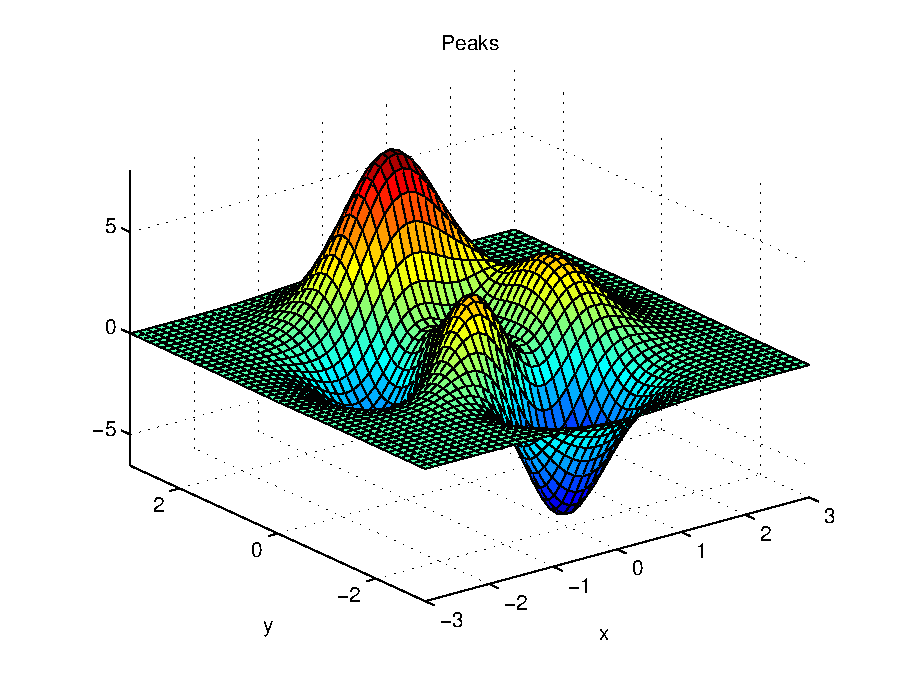
\includegraphics[width=12cm]{mcmthesis-aaa.eps}
\caption{dadasdasdd} \label{fig:aa}
\end{figure}

\eqref{aa}
\begin{equation}
a^2 \label{aa}
\end{equation}

$
  \begin{pmatrix}{*{20}c}
  {a_{11} } & {a_{12} } & {a_{13} }  \\
  {a_{21} } & {a_{22} } & {a_{23} }  \\
  {a_{31} } & {a_{32} } & {a_{33} }  \\
  \end{pmatrix}
  = \frac{{Opposite}}{{Hypotenuse}}\cos ^{ - 1} \theta \arcsin \theta
$


\[
  p_{j}=\begin{cases} 0,&\text{if $j$ is odd}\\
  r!\,(-1)^{j/2},&\text{if $j$ is even}
  \end{cases}
\]



\[
  \arcsin \theta  =
  \mathop{{\int\!\!\!\!\!\int\!\!\!\!\!\int}\mkern-31.2mu
  \bigodot}\limits_\varphi
  {\mathop {\lim }\limits_{x \to \infty } \frac{{n!}}{{r!\left( {n - r}
  \right)!}}} \eqno (1)
\]
\subsubsection{The model result}

\section{Calculating and Simplifying the Model }



\section{Validating the Model}
\subsubsection{The influences of the model}
\qquad We use the contral variable method
\begin{table}
\begin{center}
{\hspace{-1in}

\fontsize{10}{12}\selectfont
\begin{minipage}{\textwidth}
\begin{tabular}[c]{c c c c}
\toprule
\multirow{2}{*}{Primary indicator} & Weight of primary    & \multirow{2}{*}{Secondary indicator} &  Weight of secondary       \\
 & indicator & & indicator \\
\addlinespace
\toprule
\addlinespace
Native speaker & 0.5 & Number of native speakers & 0.2 \\
\addlinespace
\hline
\addlinespace
\multirow{2}{*}{Economy}    & \multirow{2}{*}{0.2} & GDP &  0.3\\
 & & FDI net & 0.2\\
\addlinespace
\hline
 \addlinespace
\multirow{3}{*}{Social culture} & \multirow{3}{*}{0.4} &  Number of official language school &  0.1\\
 & &Immigration & 0.05\\

 & &Language on internet &0.09\\
\addlinespace
\bottomrule
\end{tabular}
\end{minipage}

}\caption[Elections in G\"{o}tefrith province, 1900--1910]{Elections in
  G\"{o}tefrith province, 1900--1910.  (Taken from \cite{chicago},
  pg.~414.)}%
\label{tab:chicago-table}
\end{center}
\end{table}


After the calculation of the Fuzzy Synthetic Evaluation Model, we obtain the global distribution of all total different languages speakers. Then we established economic model to choose the place to open a office.
The model cosider the business effect and the profits that the company may receive.


\subsection{Growth of native speaker model}
\qquad We build up this model based on Fuzzy Synthetic Evaluation Model
\begin{table}
\begin{center}
{\hspace{-2in}
\begin{minipage}{\textwidth}
\fontsize{10}{12}\selectfont
\begin{tabular}[c]{lrrrrrr}
\toprule
              & \multicolumn{2}{c}{1900} & \multicolumn{2}{c}{1906} & \multicolumn{2}{c}{1910}\\
\cmidrule(r){2-3}\cmidrule(lr){4-5}\cmidrule(l){6-7}
Party         & \% of Vote  & Seats Won  & \% of Vote  & Seats Won  & \% of Vote  & Seats Won \\
\midrule
\addlinespace
              & \multicolumn{6}{c}{Provincial Assembly}\\
\cmidrule{2-7}
Conservative  & 35.6        &  47        & 26.0        & 37         & 30.9        & 52\\
Socialist     & 12.4        &  18        & 27.1        & 44         & 24.8        & 39\\
Christian Democrat & 49.2   &  85        & 41.2        & 68         & 39.2        & 59\\
Other         & 2.8         &  0         & 5.7         & 1          & 5.1         & 0\\
\addlinespace
Total& 100.0       &  150       & 100.0       & 150        & 100.0       & 150\\
\addlinespace
              & \multicolumn{6}{c}{National Assembly}\\
\cmidrule{2-7}
Conservative  & 32.6        &   4        & 23.8        &  3         & 28.3        & 3\\
Socialist     & 13.5        &   1        & 27.3        &  3         & 24.1        & 2\\
Christian Democrat & 52.0   &   7        & 42.8        &  6         & 46.4        & 8\\
Other         & 1.8         &   0        & 6.1         &  0         & 1.2         & 0\\
\addlinespace
Total& 100.0       &  12        & 100.0       & 12         & 100.0       & 13\\
\bottomrule
\end{tabular}
\end{minipage}
}
\caption[Elections in G\"{o}tefrith province, 1900--1910]{Elections in
  G\"{o}tefrith province, 1900--1910.  (Taken from \cite{chicago},
  pg.~414.)}%
\label{tab:chicago-table}
\end{center}
\end{table}

\section{Conclusions}



\section{Evaluate of the Model}

\section{Strengths and weaknesses}


\subsection{Strengths}
\begin{itemize}
\item \textbf{Applies widely}\\
This  system can be used for many types of airplanes, and it also
solves the interference during  the procedure of the boarding
airplane,as described above we can get to the  optimization
boarding time.We also know that all the service is automate.
\item \textbf{Improve the quality of the airport service}\\
Balancing the cost of the cost and the benefit, it will bring in
more convenient  for airport and passengers.It also saves many
human resources for the airline. \item \textbf{}
\end{itemize}
\cite{chicago}
\subsection{Weaknesses}
\begin{itemize}
\item \textbf{Policy never change}\\
The model works only depand on no any outside force disturb, for instance: Policy won't change, and 
wherever is stable.
\item \textbf{Data insufficient}\\

\end{itemize}
\newpage 
\section{Memo}
\begin{center}
\large {\textbf {MEMORANDUM}}
\end{center}
\textbf {To}: Chief Operating Officer \\
\textbf {From}: Team \#84802 \\
\textbf {Subject}: The best location to open office \\
\textbf {Date}: February 13,2018 \\
\noindent\rule[0.25\baselineskip]{\textwidth}{1pt}
\paragraph{} 

\bibliographystyle{plain}
\bibliography{mcm}

\begin{appendices}

\section{First appendix}


Here are simulation programmes we used in our model as follow.

\textbf{\textcolor[rgb]{0.98,0.00,0.00}{Input matlab source:}}
\lstinputlisting[language=Matlab]{./code/mcmthesis-matlab1.m}

\section{Second appendix}

some more text \textcolor[rgb]{0.98,0.00,0.00}{\textbf{Input C++ source:}}
\lstinputlisting[language=C++]{./code/mcmthesis-sudoku.cpp}

\end{appendices}

\end{document}

%% 
%% This work consists of these files mcmthesis.dtx,
%%                                   figures/ and
%%                                   code/,
%% and the derived files             mcmthesis.cls,
%%                                   mcmthesis-demo.tex,
%%                                   README,
%%                                   LICENSE,
%%                                   mcmthesis.pdf and
%%                                   mcmthesis-demo.pdf.
%%
%% End of file `mcmthesis-demo.tex'.
